\chapter{ Cl\^{o}ture du projet }
\section{Introduction}

Apr\`{e}s avoir fini avec la conception de l'application,nous allons entamer la
partie r\'{e}alisation et impl\'{e}mentation dans laquelle on s'assure que le
syst\`{e}me est pr\^{e}t pour \^{e}tre exploit\'{e} par les utilisateurs finaux.
A la fin de ce chapitre, les objectifs doivent avoir \'{e}t\'{e} atteints et le projet doit
\^{e}tre clos.
Vous pouvez trouvez l'application sur le lien [13].


  Pour acc\'{e}der en tant qu'administrateur veuiilez utiliser:

  \begin{itemize}
    \item {\textbf{ Pseudo:}admin}
    \item {\textbf{ Password:}0000}
  \end{itemize}


  Pour acc\'{e}der en tant que membre 'Wael Chorfan' par exemple veuillez utiliser:

  \begin{itemize}
    \item {\textbf{ Pseudo:}WC}
    \item {\textbf{ Password:}0001}
  \end{itemize}

 \newpage

\section{Environnement de d\'{e}veloppement}


  \subsection{Languages used}


  chmengui page 53
  \textbf{JSON}\newline

JSON (JavaScript Object Notation) est un format de données textuel, géné-
rique, dérivé de la notation des objets du langage ECMAScript. Il permet de re-
présenter de l’information structurée [13]. Un document JSON ne comprend que
deux éléments structurels :
– des ensembles de paires nom / valeur .
– des listes ordonnées de valeurs.
Ces mêmes éléments représentent 3 types de données :
– des objets;
– des tableaux;
– des valeurs génériques de type tableau, objet, booléen, nombre, chaîne ou
null.


Node js
Framework javascript ,nous l'avons utilis\'{e} pour cr\'{e}er le serveur web .
Il offre la rapidit\'{e} de ,la performance etla modularit\'{e}.
\bigskip


\textbf{ Express js:}
framework node js qui sert \`{a} cre\'{e}r l'application ,il est en
relation avec la base de donn\'{e}es par le biais de driver mysql et en relation
avec les modules web par le moteur de vues EJS.
\bigskip
\textbf{ Vue js:}

Framework javascript front-end utilis\'{e} pour la programmation et la
manipulation des actions,entr\'{e}es et sorties des diff\'{e}rents modules .
\bigskip

\textbf{ Mysql:}
Langage de la base de donn\'{e}es relationnelle utilis\'{e}e.
e.EJS moteur de vue d'express js , ce type permet l'intercommunication entre
les modules web et le serveur .
\bigskip

\textbf{ EJS:}
moteur de vue d'express js , ce type permet l'intercommunication entre
les modules web et le serveur .
\bigskip


\textbf{ Highcharts: }
L'outil de \guillemotleft{} reporting \guillemotright{} sur des pages web
\bigskip





Express js la base de l'application web ,il nous permet de cr\'{e}er l'API REST
qui nous permet de distribuer les elements de l'applications sur des \guillemotleft{} routes \guillemotright{}
ou nous pouvons les acc\'{e}der \`{a} l'aide des middlewares express .
L'authentification est donc faite par un contr\^{o}le sur certains \guillemotleft{} routes \guillemotright{}.
Les middlewarent permettent de communiquer les param\'{e}tres d'entr\'{e}e sortie
entre les pages web d'une part et autres la base de donn\'{e}es d'autre part.

\newpage


\subsection{env materiel }
Pour la r\'{e}alisation du projet, nous avons utilis\'{e} :
1. Un ordinateur portable pour le d\'{e}veloppement ayant les caract\'{e}ristiques suivantes :
\textendash{} Mod\`{e}le : Asus XJ550.
\textendash{} Processeur : i7 2.6GHz.
\textendash{} Disque Dur : 1To
\textendash{} Syst\`{e}mes d'exploitation : Windows 7.
– M\'{e}moire : 8Go.


\subsection{env logiciel}
vs code et wamp [1] [2] ...
vue js extension
power bi
talend
postman




\section{Impl\'{e}mentation et structure}

Les \'{e}tapes \'{e}taient :
\bigskip

\begin{itemize}
\item{ Cr\'{e}er le site web statique (front -end) }
\\~~
\item{Cr\'{e}er une application express js }
\\~~
\item{  Cr\'{e}ation du base de donn\'{e}es et liaison des donn\'{e}es par le driver node js
de mysql}
\\~~
\item{Cr\'{e}er un rest api \`{a} l'aide de express js }
\\~~
\item{Int\'{e}gration de front-end avec le back-end }
\\~~
\item{Ajout des modules suppl\'{e}mentaire (Authentification avec jwt et gestion
des roles utilisateur et administrateur) }
\\~~
\item{ H\'{e}bergement en ligne de la base de donn\'{e}es}
\\~~
\item{ H\'{e}bergement en ligne de l'application web}
\\~~
\end{itemize}



Nous allons diviser cette partie par pr\'{e}senter les fonctionnalit\'{e}s offertes par
l'application :
Rq : Les donn\'{e}es et les noms sont virtuelles pour des raisons de test .



Si un simple membre est authentifi\'{e} par son mot de passe il sera amen\'{e}e \`{a}
l'interface \guillemotleft{} gestion de taches \guillemotright{} dans laquelle il peut modifier l'\'{e}tat des
taches .(ToDo ,Doing,Done ) et La progression des taches .

\FloatBarrier
\begin{figure}[H]
\center
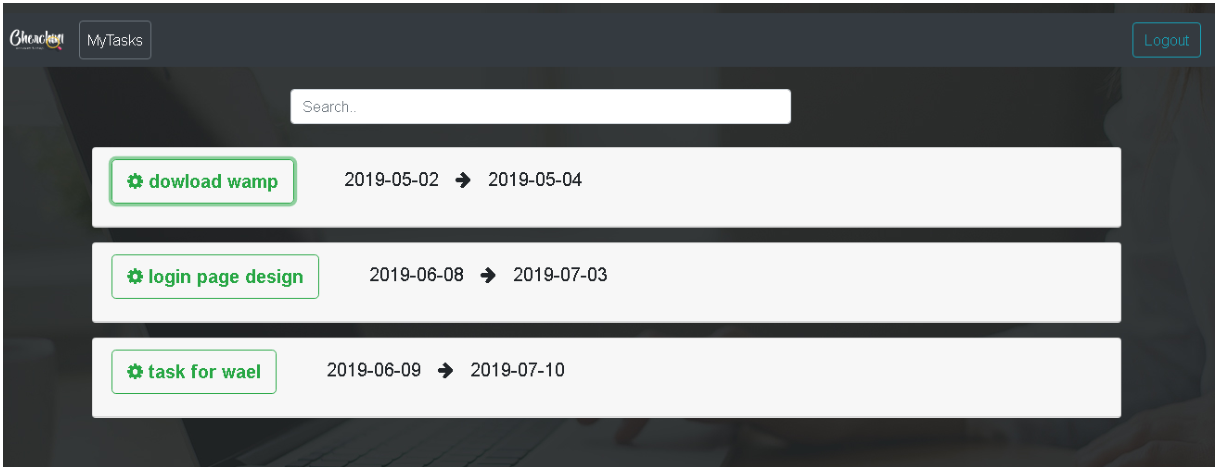
\includegraphics[width=11cm,height=7cm]{./figures/pres/2.png}
\caption{Espace membre.1.}

\end{figure}
\FloatBarrier

\FloatBarrier
\begin{figure}[H]
\center
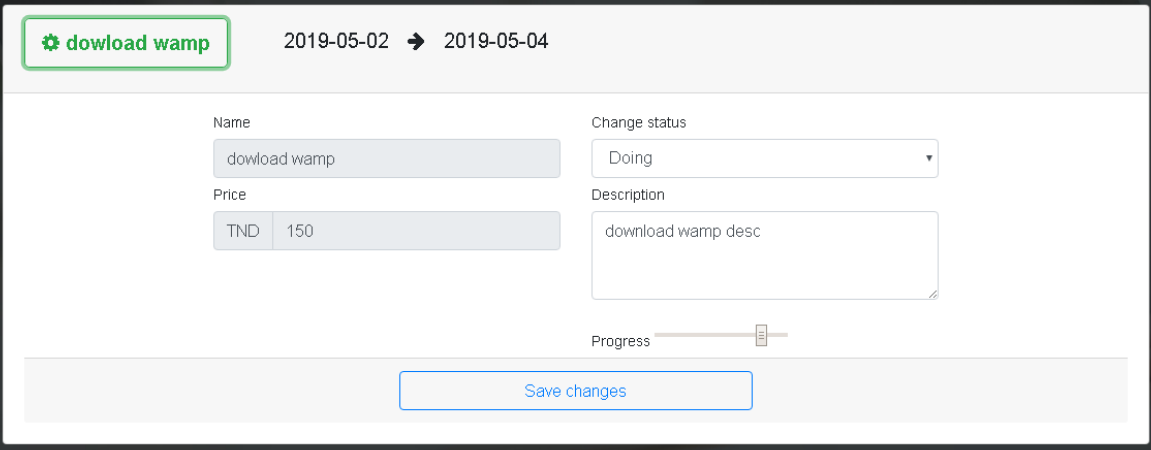
\includegraphics[width=11cm,height=7cm]{./figures/pres/3.png}
\caption{Espace membre.2.}

\end{figure}
\FloatBarrier
\subsection{Acc\'{e}es Administrateur}

Si l'administrateur parvient \`{a} ese connecter il trouve cette interface d'accueil
ou il trouvera les rapports qui d\'{e}crivent des statistiques primordiales au
d\'{e}oulement des projets donc les interfaces et les fonctionnalit\'{e}s disponibles
pour l'admin sont :

\subsection{La consultation des rapports}


\FloatBarrier
\begin{figure}[H]
\center
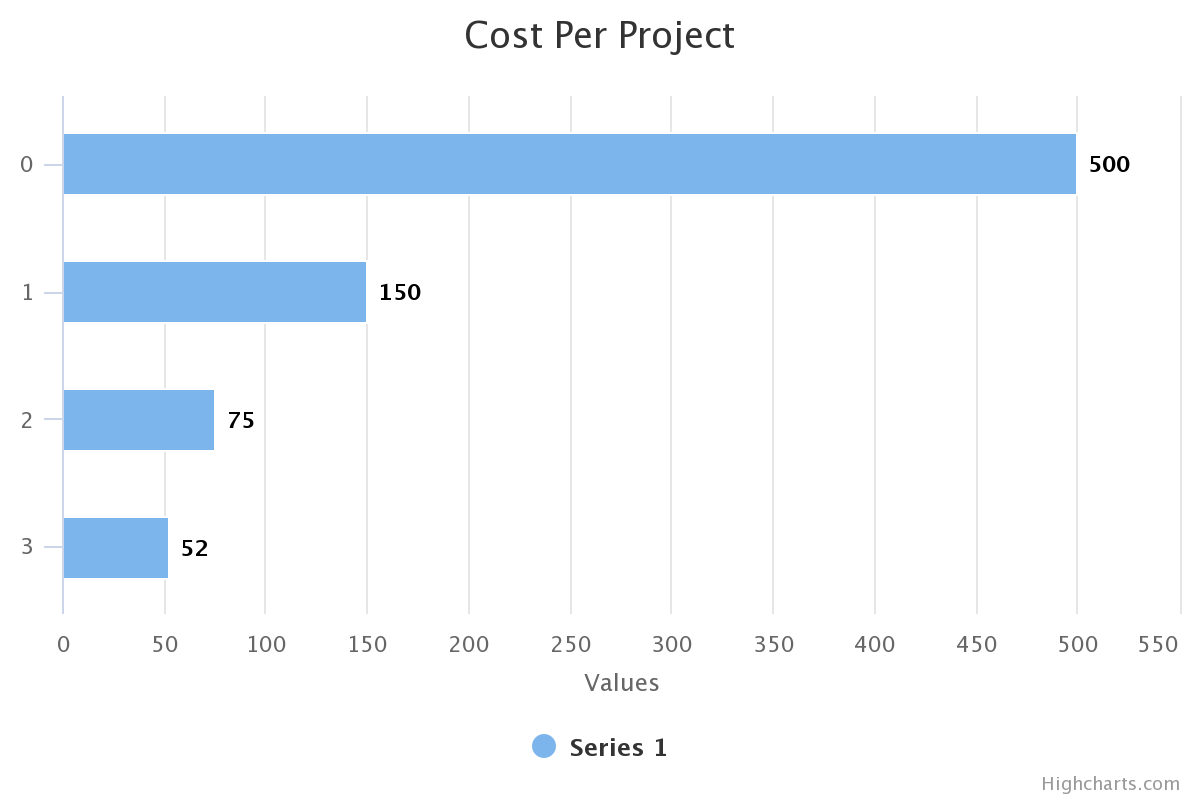
\includegraphics[width=11cm,height=7cm]{./figures/pres/cost-per-project.png}
\caption{ Co\^{u}t par projet }
\end{figure}
\FloatBarrier

\FloatBarrier
\begin{figure}[H]
\center
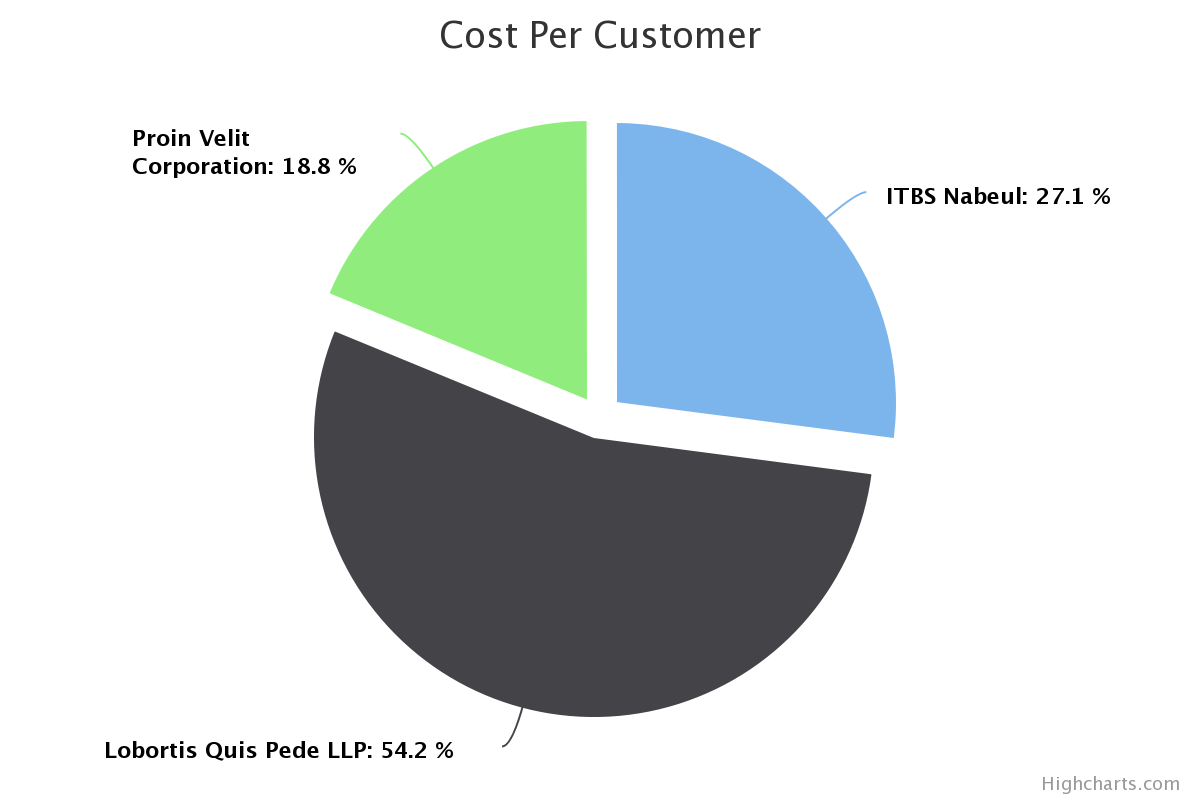
\includegraphics[width=11cm,height=7cm]{./figures/pres/cost-per-customer.png}
\caption{ Co\^{u}t par client }
\end{figure}
\FloatBarrier

\FloatBarrier
\begin{figure}[H]
\center
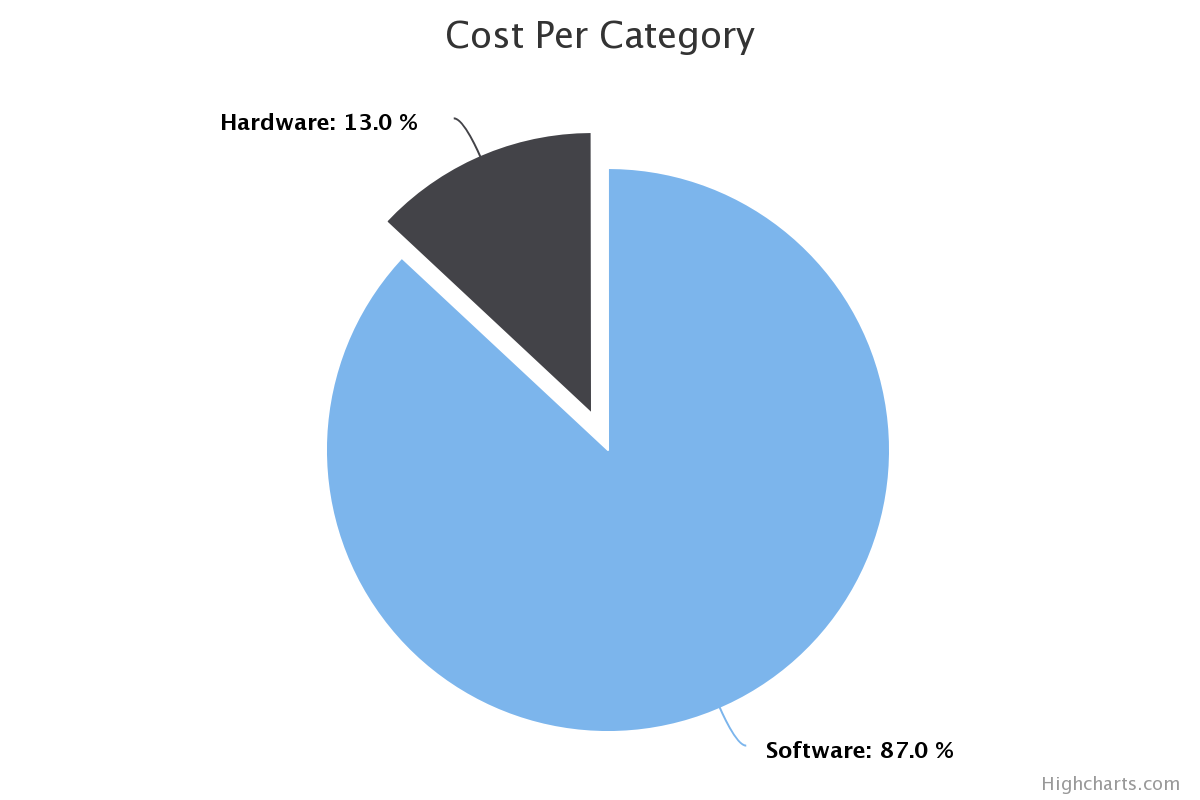
\includegraphics[width=11cm,height=7cm]{./figures/pres/cost-per-category.png}
\caption{ Co\^{u}t par cat\'{e}gorie}
\end{figure}
\FloatBarrier

\FloatBarrier
\begin{figure}[H]
\center
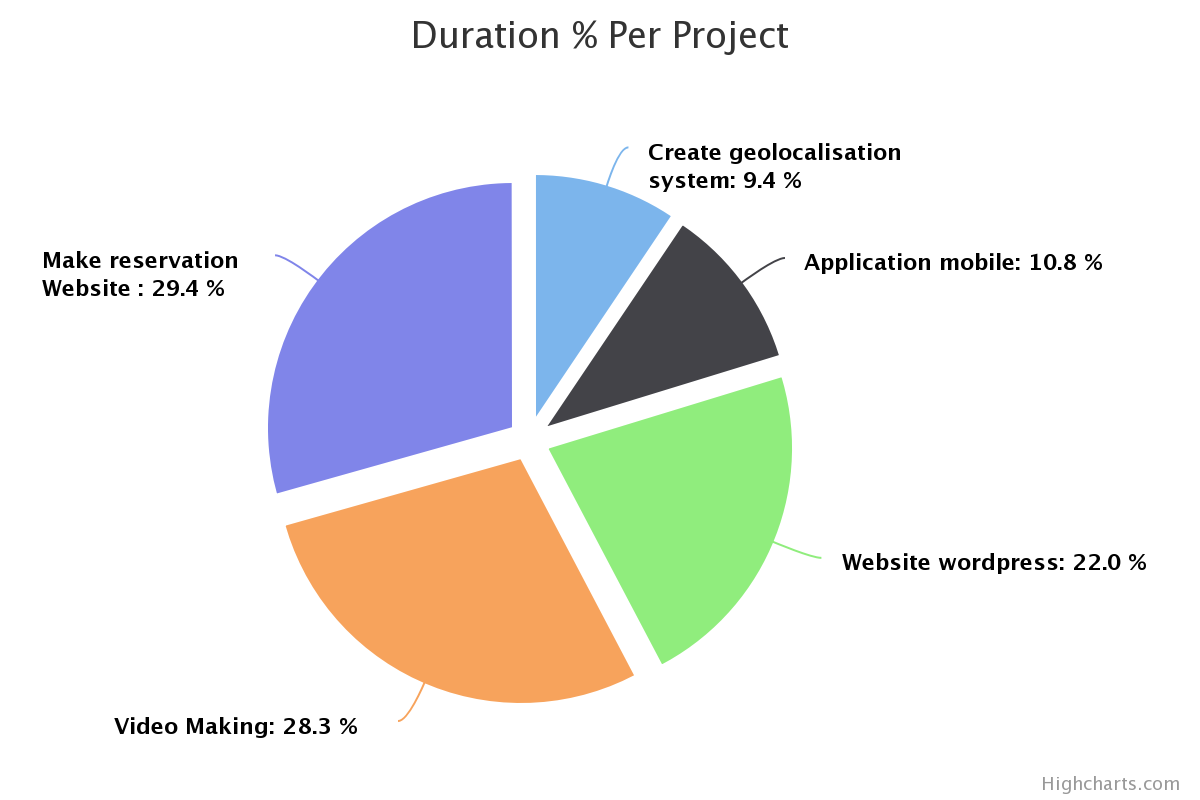
\includegraphics[width=11cm,height=7cm]{./figures/pres/duration-per-project.png}
\caption{Dur\'{e}e par projet.1. }
\end{figure}
\FloatBarrier

\FloatBarrier
\begin{figure}[H]
\center
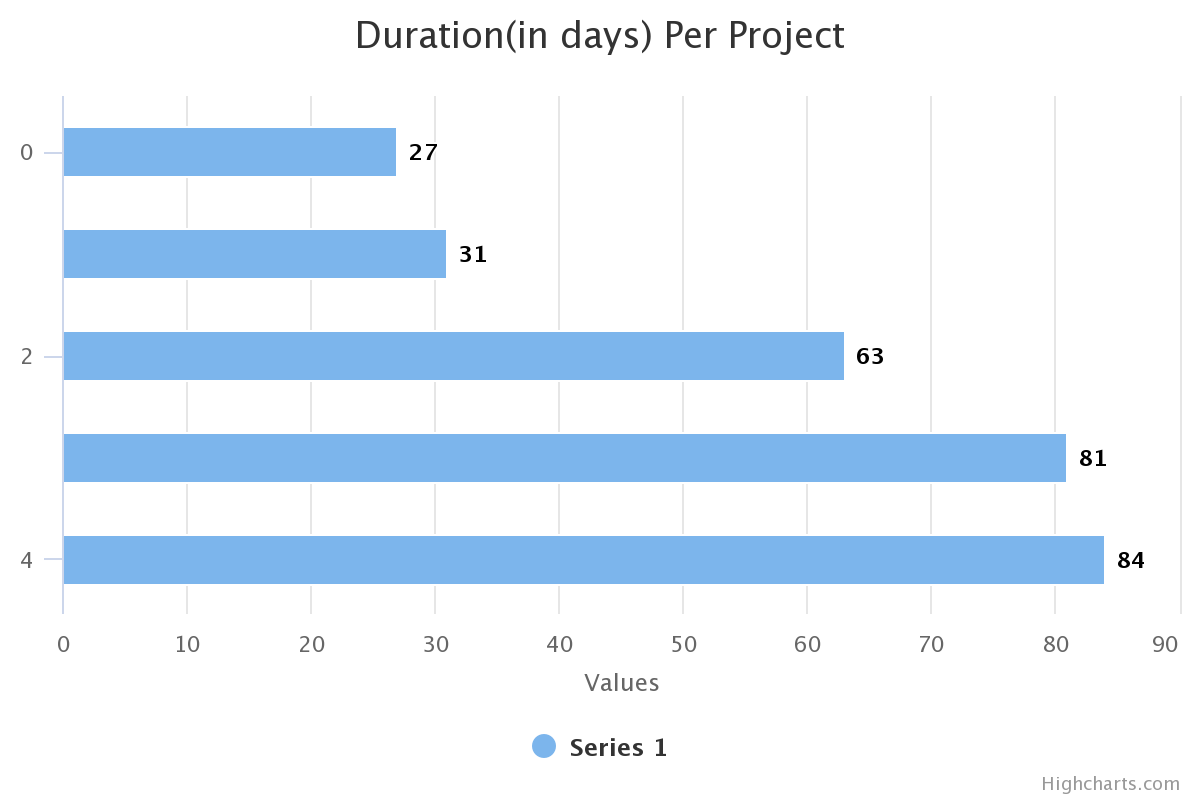
\includegraphics[width=11cm,height=7cm]{./figures/pres/durationin-days-per-proj.png}
\caption{Dur\'{e}e par projet.2.}
\end{figure}
\FloatBarrier









\newpage






